% Cosmic Microwave Background Radiation
%
%  Data taken from: http://map.gsfc.nasa.gov/m_uni/uni_101bbtest3.html
%
% This file is included from ranges.tex
%
%Unit description from: http://www.unc.edu/~rowlett/units/
%Intensity measured in MJy/sr
%jansky (Jy)    a unit used in radio astronomy to measure the strength, or more precisely the flux density, of radio signals from space. In measuring signal strength, it's necessary to take into account both the area of the receiving antenna and the width of the frequency band in which the signal occurs. Accordingly, one jansky equals a flux of 10-26 watts per square meter of receiving area per hertz of frequency band (W/m2Hz). Although it is not an SI unit, the jansky is approved by the International Astronomical Union and is widely used by astronomers. It honors Karl G. Jansky (1905-1950), the American electrical engineer who discovered radio waves from space in 1930. The jansky is sometimes called the flux unit.
%steradian (sr)     the standard unit of solid angle measure in mathematics. Just as there are 2pi radians in a circle, there are 4pi steradians in a sphere. Thus one steradian equals about 0.079 577 sphere. There are 129 600/pi = 41 252.96 square degrees in a sphere, so 1 steradian also equals about 3282.806 square degrees. The unit originated in the 1870s by analogy with the radian.
%
%\pscurve[fillstyle=none](.25,20.96)(.125,21.27)(.01625,21.61)(.05,21.77)(.25,22.06)(.39375,22.27)(.4625,22.43)(.4875,22.56)
%\psaxes[linecolor=white, labels=x](.5,2)
\psclip{\psframe[fillstyle=none,linewidth=1pt,linecolor=white](0,0)(.5,1.6)}
  \definecolor{Fill}{rgb}{0.9,0.1,0.67}
  \pscurve[fillstyle=hlines,hatchcolor=Fill,hatchangle=0,hatchwidth=0.2pt,hatchsep=1pt,fillcolor=blue,linecolor=Fill]
	(0.5,-1)(.25,0)(.125,.31)(.01625,.65)(.05,.81)(.25,1.1)(.39375,1.31)(.4625,1.47)(.4875,1.6)
  \rput{90}(.3,.6){\white T=2.725\kelvin}
  \rput(.25,1.5){\white CMB}
\endpsclip
{\textcolor{white}{
 \uput[r](.5,0){65 GHz}
 \uput[r](.5,1.6){600 GHz}
 \uput[d]{90}(0,0){400 MJy/sr}
 \uput[d]{90}(.5,0){0 MJy/sr}
 \uput[d]{90}(.25,0){Intensity}
 \psline[linecolor=FColor]{<-}(.5,.8)(1.2,.8)
 \uput[r](1.1,.55){\psframebox[cornersize=absolute,linearc=4pt,fillstyle=solid,fillcolor=Black, linecolor=white]
   	{\parbox[t]{3.74in}{\white
	{\Large {\bfseries C}osmic {\bfseries M}icrowave {\bfseries B}ackground Radiation}
		\begin{itemize}
			% By Douglas Scott
			\item  CMB radiation is the leftover heat from the hot early universe, which last scattered about 400,000 years after the Big Bang.
			%\item  CMR is the leftover heat emitted 400,000 years after the big bang.
			\item  CMB permeates the entire universe at a temperature of 2.725 $\pm$ 0.001\kelvin.
			%prediction statement removed based on http://www.dfi.uem.br/~macedane/history_of_2.7k.html which complicates the issue too much
			% By Douglas Scott
			%\item  CMB was predicted in the 1940's by Ralph Alpher, George Gamow and Robert Herman.
			% original
			%\item  George Gamow predicted CMB in 1948 and Ralph Alpher and Robert Herman in 1950.
			\item  Arno Penzias and Robert Wilson accidentally discovered CMB while working for Bell Telephone Laboratories in 1965.
			\item  The intensity is measured in Mega Jansky ($Jy$) per steradian. $1 Jy  = 10^{-26} W/m^2/Hz$
		\end{itemize}
	\vspace{0.1in}
	%
	% According to http://nix.nasa.gov/copyright.html the CMB image at http://map.gsfc.nasa.gov/m_mm.html
	%
	\begin{tabular}{rl}
	\begin{minipage}[b]{1.05in}\rput(.65,.3){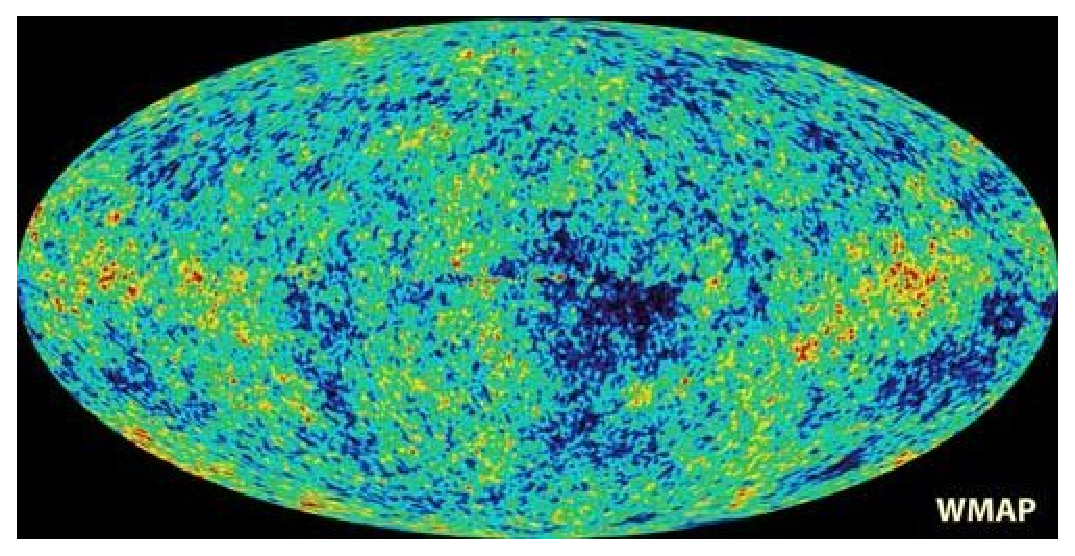
\includegraphics[width=1in]{pictures/wmap.eps}}
	\end{minipage}&
	\hspace{0.0in}
	\begin{minipage}[b]{2.4in}\textcolor{white}{%
	Close examination of slight CMB intensity variations in different parts of the sky help cosmologists study the formation of galaxies.
	\textcolor{gray}{WMAP photo by NASA}
	}
	\end{minipage}
	\end{tabular}
	}
	}
	}
}}
